\documentclass{article}
\usepackage{tikz}

\begin{document}

\begin{figure}[h]
    \centering
    \begin{subfigure}{0.45\textwidth}
        \caption{}
        \label{fig:a}
        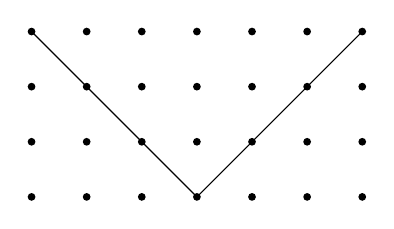
\begin{tikzpicture}[scale=0.7]
            % Draw points
            \foreach \x in {0,...,6} {
                \foreach \y in {0,...,3} {
                    \fill (\x,\y) circle (2pt);
                }
            }
            % Draw lines
            \draw (0,3) -- (3,0) -- (6,3);
        \end{tikzpicture}
    \end{subfigure}
    \hfill
    \begin{subfigure}{0.45\textwidth}
        \caption{}
        \label{fig:b}
        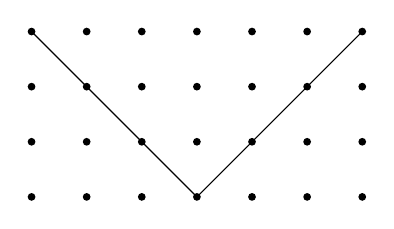
\begin{tikzpicture}[scale=0.7]
            % Draw points
            \foreach \x in {0,...,6} {
                \foreach \y in {0,...,3} {
                    \fill (\x,\y) circle (2pt);
                }
            }
            % Draw lines
            \draw (0,3) -- (3,0) -- (6,3);
        \end{tikzpicture}
    \end{subfigure}
\end{figure}

\end{document}